\section{Behavior, Interaction and Priority (BIP)}
\label{sec:bip}
We recall the necessary concepts of the BIP framework~\cite{bip2}.
BIP allows to construct systems by superposing three layers of design: Behavior, Interaction, and Priority.
The \emph{behavior} layer consists of a set of atomic components represented by transition systems. 
The \emph{interaction} layer provides the collaboration between components. 
Interactions are described using sets of ports. 
The \emph{priority} layer is used to specify scheduling policies applied to the interaction layer, given by a strict partial order on interactions.

\subsection{Atomic Components}
We define \emph{atomic components} as transition systems with a set of ports labeling individual transitions. These ports are used for communication between different components.

\begin{definition}[Atomic Component]
An  {\em atomic component} $B$ is a labeled transition system represented by a triple $(Q,P,\goesto)$ where $Q$ is a set of {\em states}, $P$ is a set of {\em communication ports}, $\goesto\, \subseteq Q\times P\times Q$ is a set of {\em possible transitions}, each labeled by some port.
\end{definition}

For any pair of states $q,q'\in Q$ and a port $p\in P$, we write $q \goesto[p] q'$, iff $(q,p,q')\in\,\goesto$. When the communication port is irrelevant, we simply write $q \goesto q'$. Similarly, $q \goesto[p]$ means that there exists $q'\in Q$ such that $q \goesto[p] q'$. In this case, we say that $p$ is \emph{enabled} in state $q$.

In practice, atomic components are extended with variables. Each variable may be
bound to a port and modified through interactions involving this port. We also
associate a guard and an update function (i.e., action) to each transition. A guard is a
predicate on variables that must be true to allow the execution of the
transition. An update function is a local computation triggered by the
transition that modifies the variables. 

Figure \ref{fig:philo-fork} shows an atomic component $P$ that corresponds to the behavior of a philosopher in the dining-philosopher problem, where $Q = \{e,h\}$ denotes eating and hungry, $P = \{\release, \get\}$ denotes releasing and getting of forks, and $\goesto = \{e \goesto[\release] h, h \goesto[\get] e\}$.


\subsection{Composition Component}
For a given system built from a set of $n$ atomic components $\{B_i = (Q_i, P_i, \goesto_i)\}_{i=1}^n$, we assume that their respective sets of ports are pairwise disjoint, i.e., for any two $i\not= j$ from $\set{1..n}$, we have $P_i \cap P_j = \emptyset$. We can therefore define the set $P = \bigcup_{i=1}^n P_i$ of all ports in the system. An {\em interaction} is a set $a \subseteq P$ of ports. When we write $a = \{p_i\}_{i\in I}$, we suppose that for $i \in I$, $p_i \in P_i$, where $I \subseteq \set{1..n}$.

Similar to atomic components, BIP extends interactions by associating a guard
and a transfer function to each of them. Both the guard and the function are defined over
the variables that are bound to the ports of the interaction. The guard must be
true to allow the interaction. When the interaction takes place, the
associated transfer function is called and modifies the variables.

\begin{figure}[t]
  \begin{center}
    \mbox{
      \subfigure[Philosopher $P$ and fork $F$ atomic components.]{\label{fig:philo-fork}\scalebox{0.35}{\input{figs/philAndFork.pdf_t}}} \quad
      \subfigure[Dining philosophers composite component with four philosophers.]{\label{fig:diningbip}\scalebox{0.3}{\input{figs/diningbip.pdf_t}}}
      }
    \caption{Dining philosophers.}
    \label{fig:diningSpectrum}
  \end{center}
\end{figure}

\begin{definition}[Composite Component]\label{def.bip.composition}
A {\em composite \linebreak component} (or simply {\em component}) is defined by a composition operator parameterized by a set of interactions $\Gamma \subseteq 2^P$.  $B \stackrel{\mathit{def}}{=} \Gamma(B_1,\dots,B_n)$, is a transition system $(Q,\Gamma, \goesto)$, where $Q=\bigotimes_{i=1}^n Q_i$ and $\goesto$ is the least set of transitions satisfying the rule

\begin{mathpar}
\inferrule
{
    a = \{p_i\}_{i\in I}\in \Gamma\\
    \forall i\in I: q_i \goesto[p_i]_i q'_i\\
    \forall i\not\in I: q_i = q'_i\\
}
{
    (q_1,\dots,q_n) \goesto[a] (q'_1,\dots,q'_n)
}
\end{mathpar}
\end{definition}

The inference rule says that a composite component $B=\Gamma(B_1,\dots,B_n)$ can
execute an interaction $a\in \Gamma$, iff for each port $p_i\in a$, the
corresponding atomic component $B_i$ can execute a transition labeled with
$p_i$; the states of components that do not participate in the interaction stay
unchanged. 

Figure~\ref{fig:diningbip} illustrates a composite component $\Gamma(P_0, P_1, P_2, P_3, F_0, F_1, F_2, F_3)$, where each $P_i$ (resp. $F_i$)  is identical to component $P$ (resp. $F$) in Figure
\ref{fig:philo-fork} and $\Gamma = \Gamma_\get \, \cup \, \Gamma_\release$, where $\Gamma_\get = \bigcup_{i=0}^{3} \{P_i.\get, F_i.\use_l, F_{(i+1) \% 4}.use_r\}$ and $\Gamma_\release = \bigcup_{i=0}^{3}\{P_i.\release, F_i.\free_l, F_{(i+1)\%4}.free_r\}$. 


Notice that several distinct interactions can be enabled at the same time, thus introducing non-determinism in the product behavior. One can add priorities to reduce non-determinism. In this case, one of the interactions with the highest priority is chosen non-deterministically.

\begin{definition}[Priority]
  \label{defn:priority}
  Let $C = (Q,\Gamma,\goesto)$ be the behavior of the composite component $\Gamma(\{B_1, \ldots, B_n\})$.  A {\em priority model} $\prio$ is a
  strict partial order on the set of interactions $\Gamma$. Given a priority model $\prio$, we
  abbreviate $(a,a')\in \prio$ by $a \prec a'$. Adding the priority model $\prio$ over $\Gamma(\{B_1, \ldots, B_n\})$ defines a new composite component $B = \prio\big(\Gamma(\{B_1, \ldots, B_n\})\big)$ noted $\pi(C)$ and whose behavior is defined by $(Q, \Gamma, \goesto_\prio)$, where $\goesto_\prio$ is the least set of transitions satisfying the following rule:
\begin{mathpar}
\inferrule*
	{
      q \goesto[a] q' \and
      \neg\big(\exists a'\in \Gamma,\exists q''\in Q: a \prec a' \wedge q \goesto[a'] q'' \big)
    }
    {
      q \goesto[a]_\prio q'
    }
\end{mathpar}
\end{definition}
%
An interaction $a$ is enabled in $\pi(C)$ whenever $a$ is enabled in $C$ and $a$ is maximal according to $\pi$ among the active interactions in $C$.


BIP provides both centralized and distributed implementations. In the centralized implementation,
a centralized engine guarantees to execute only one interaction at a time, and thus conforms to the operational semantics of the BIP.  The main loop of the BIP engine consists of the following steps:
\begin{enumerate}
\item Each atomic component sends to the engine its current
location.
\item The engine enumerates the list of interactions in the system,
selects the enabled ones based on the current location
of the atomic components and eliminates the ones
with low priority.
\item The engine non-deterministically selects an interaction
out of the enabled interactions.
\item Finally, the engine notifies the corresponding components
and schedules their transitions for execution.
\end{enumerate}

Alternatively, BIP allows the generation of distributed
implementations~\cite{bip-distributed} where non-conflicting interactions
can be simultaneously executed.

\begin{definition}[BIP system]
\label{def:bipsystem}
A BIP system is a tuple $(B, q_0)$, where $q_0$ is the initial state with $q_0 \in \bigotimes_{i=1}^n Q_i$ being the tuple of initial states of atomic components.
\end{definition}


For the rest of the paper, we fix an arbitrary BIP-system $(B, q_0)$, where  $B = \prio\big(\Gamma(\{B_1, \ldots, B_n\})\big)$ with semantics $C = (Q, \Gamma, \goesto)$.

We abstract the execution of a BIP system as a trace.
%
\begin{definition}[BIP trace]
\label{def:trace-global}
A BIP trace $\rho = (q_0 \cdot a_0 \cdot q_1 \cdot a_1 \cdots q_{i-1} \cdot a_{i-1} \cdot q_i)$ is an alternating sequence of states of $Q$ and interactions in $\Gamma$; where $q_k \xrightarrow{a_k} q_{k+1} \in \rightarrow$, for $k \in [0, i-1]$.
\end{definition}

Given a trace $\rho = (q_0 \cdot a_0 \cdot q_1 \cdot a_1 \cdots q_{i-1} \cdot a_{i-1} \cdot q_i)$, 
$\rho^q_i$ (resp. $\rho^a_i$) denotes the $i^\text{th}$ state (resp. interaction) of the trace, i.e., $q_i$ (resp. $a_i$). Also, $\bm{\rho}(C)$ denotes the set of all the traces of an LTS $C$. 

\section{Neural Networks}
We use a neural networks to model the behavioral function of the agent in the infinite setting. In this section, we briefly review these forms. 


Neural Networks (NNs) were originally motivated by looking at machines which replicate the brain's functionality. In an artificial neural network, a neurone is a logistic unit, which is fed inputs through input wires. This unit can perform computations resulting in outputs that are transmitted through the output wires. 

\begin{figure}[h!]
\label{Fig:FigOne}
\centering 
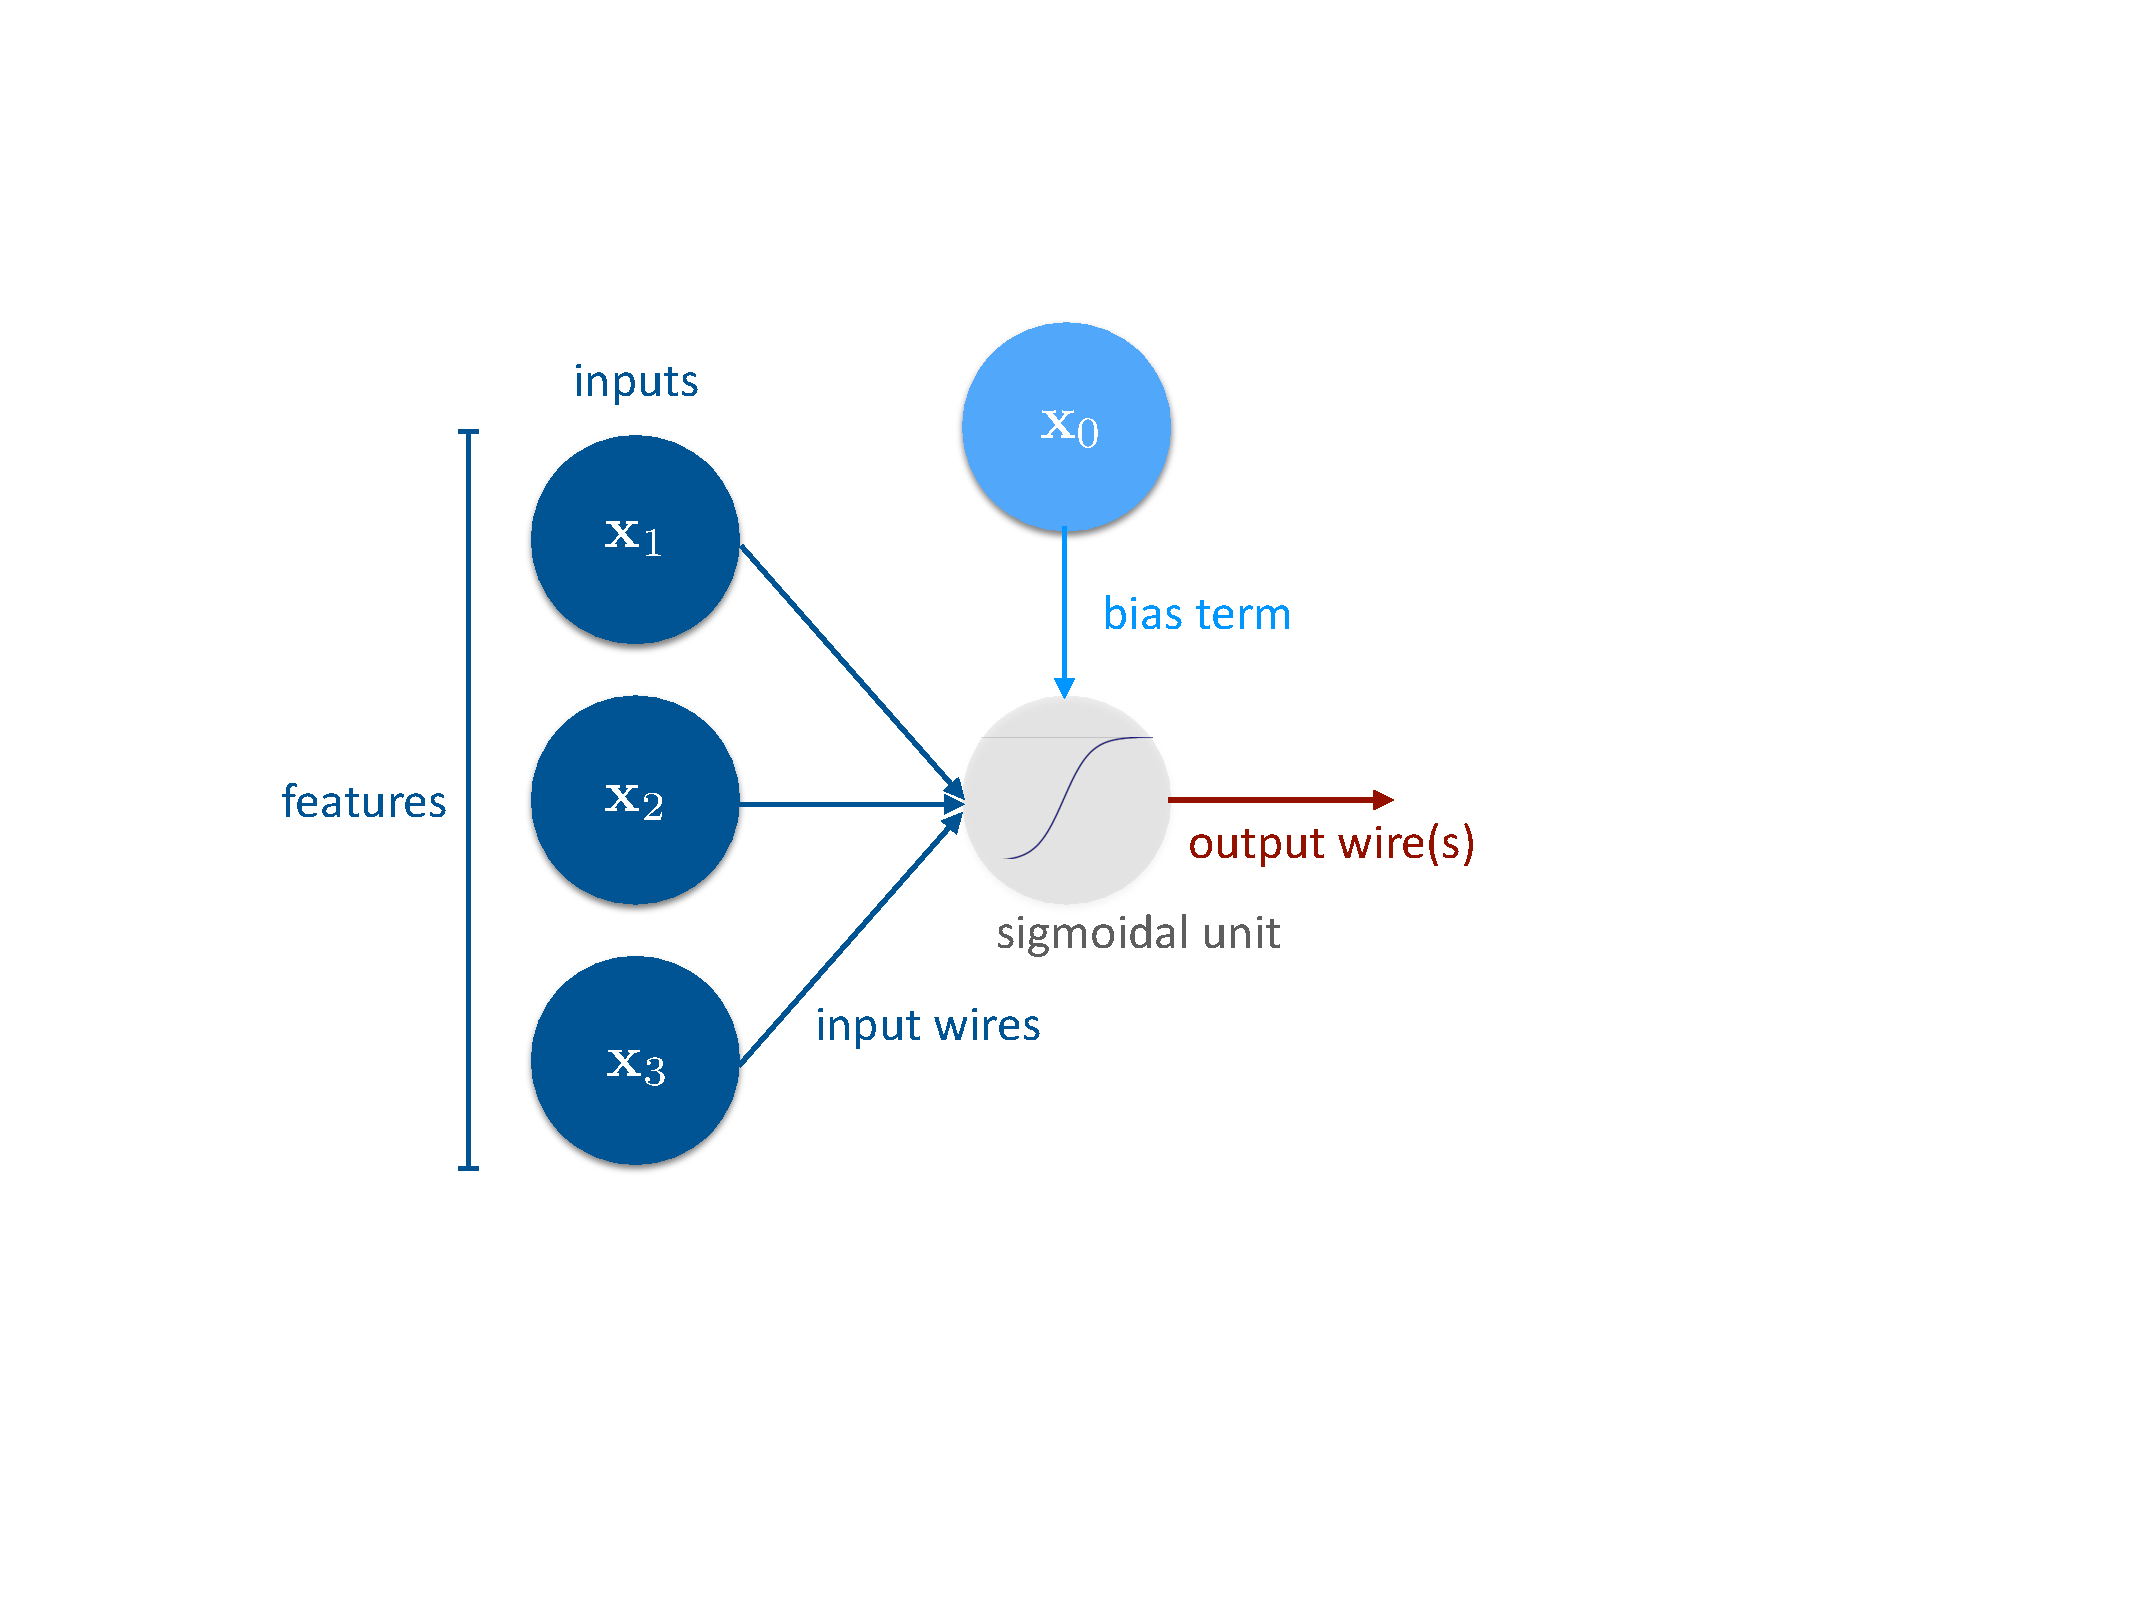
\includegraphics[trim = 10em 10em 10em 10em, clip, width= .7\textwidth]{OneUnit}
\caption{A high-level depiction of a logistic unit showing the: 1) inputs with their input wires, 2) nonlinear sigmoidal transformation, and 3) the output wires. }
\end{figure}

An illustration of a single neurone is shown in Figure~\ref{Fig:FigOne} for a three dimensional input vector $\bm{x} = [x_{1}, x_{2}, x_{3}]^{\mathsf{T}}$, and an appended bias term $x_{0}$. In the logistic unit, the input vector is first linearly combined using a weight vector, $\bm{\theta}$, and then nonlinearly transformed using a sigmoidal function. Consequently, the output delivered on the output wire can be written as:
\begin{equation*}
h_{\bm{\theta}} (\bm{x}) = \frac{1}{1 + e^{-\bm{\theta}^{\mathsf{T}}}\bm{x}} = \frac{1}{1 + e^{-\sum_{i=0}^{3} \theta_{i}x_{i}}},
\end{equation*}
with $x_{0} =1$ denoting the bias term, and $\bm{\theta} = [\theta_{0}, \theta_{1}, \theta_{2}, \theta_{3}]^{\mathsf{T}}$ representing the weights connecting the inputs. 

An artificial neural network is simply a set of these logistic units strung together as shown in Figure~\ref{Fig:FigTwo}. Each two layers are connected together using weight parameters. As such, the neural network in Figure~\ref{Fig:FigTwo} possesses two weighting matrices, $\bm{\Theta}^{(1)}$ and $\bm{\Theta}^{(2)}$. Here, we used $\bm{\Theta}^{(l)}$ to denote the weights connecting layers $l$ and $l+1$. Definitely, the dimensionality of $\bm{\Theta}^{(l)}$ depends on the number of units in each of the two layers. For example, if layer $l$ consists of $s_{l}$ units and layer $l+1$ of $s_{l+1}$, $\bm{\Theta}^{(l)}$ has a dimensionality of $s_{l+1} \times s_{l} +1$, where we have added another dimension to incorporate the bias term. 

\begin{figure}[h!]
\label{Fig:FigTwo}
\centering 
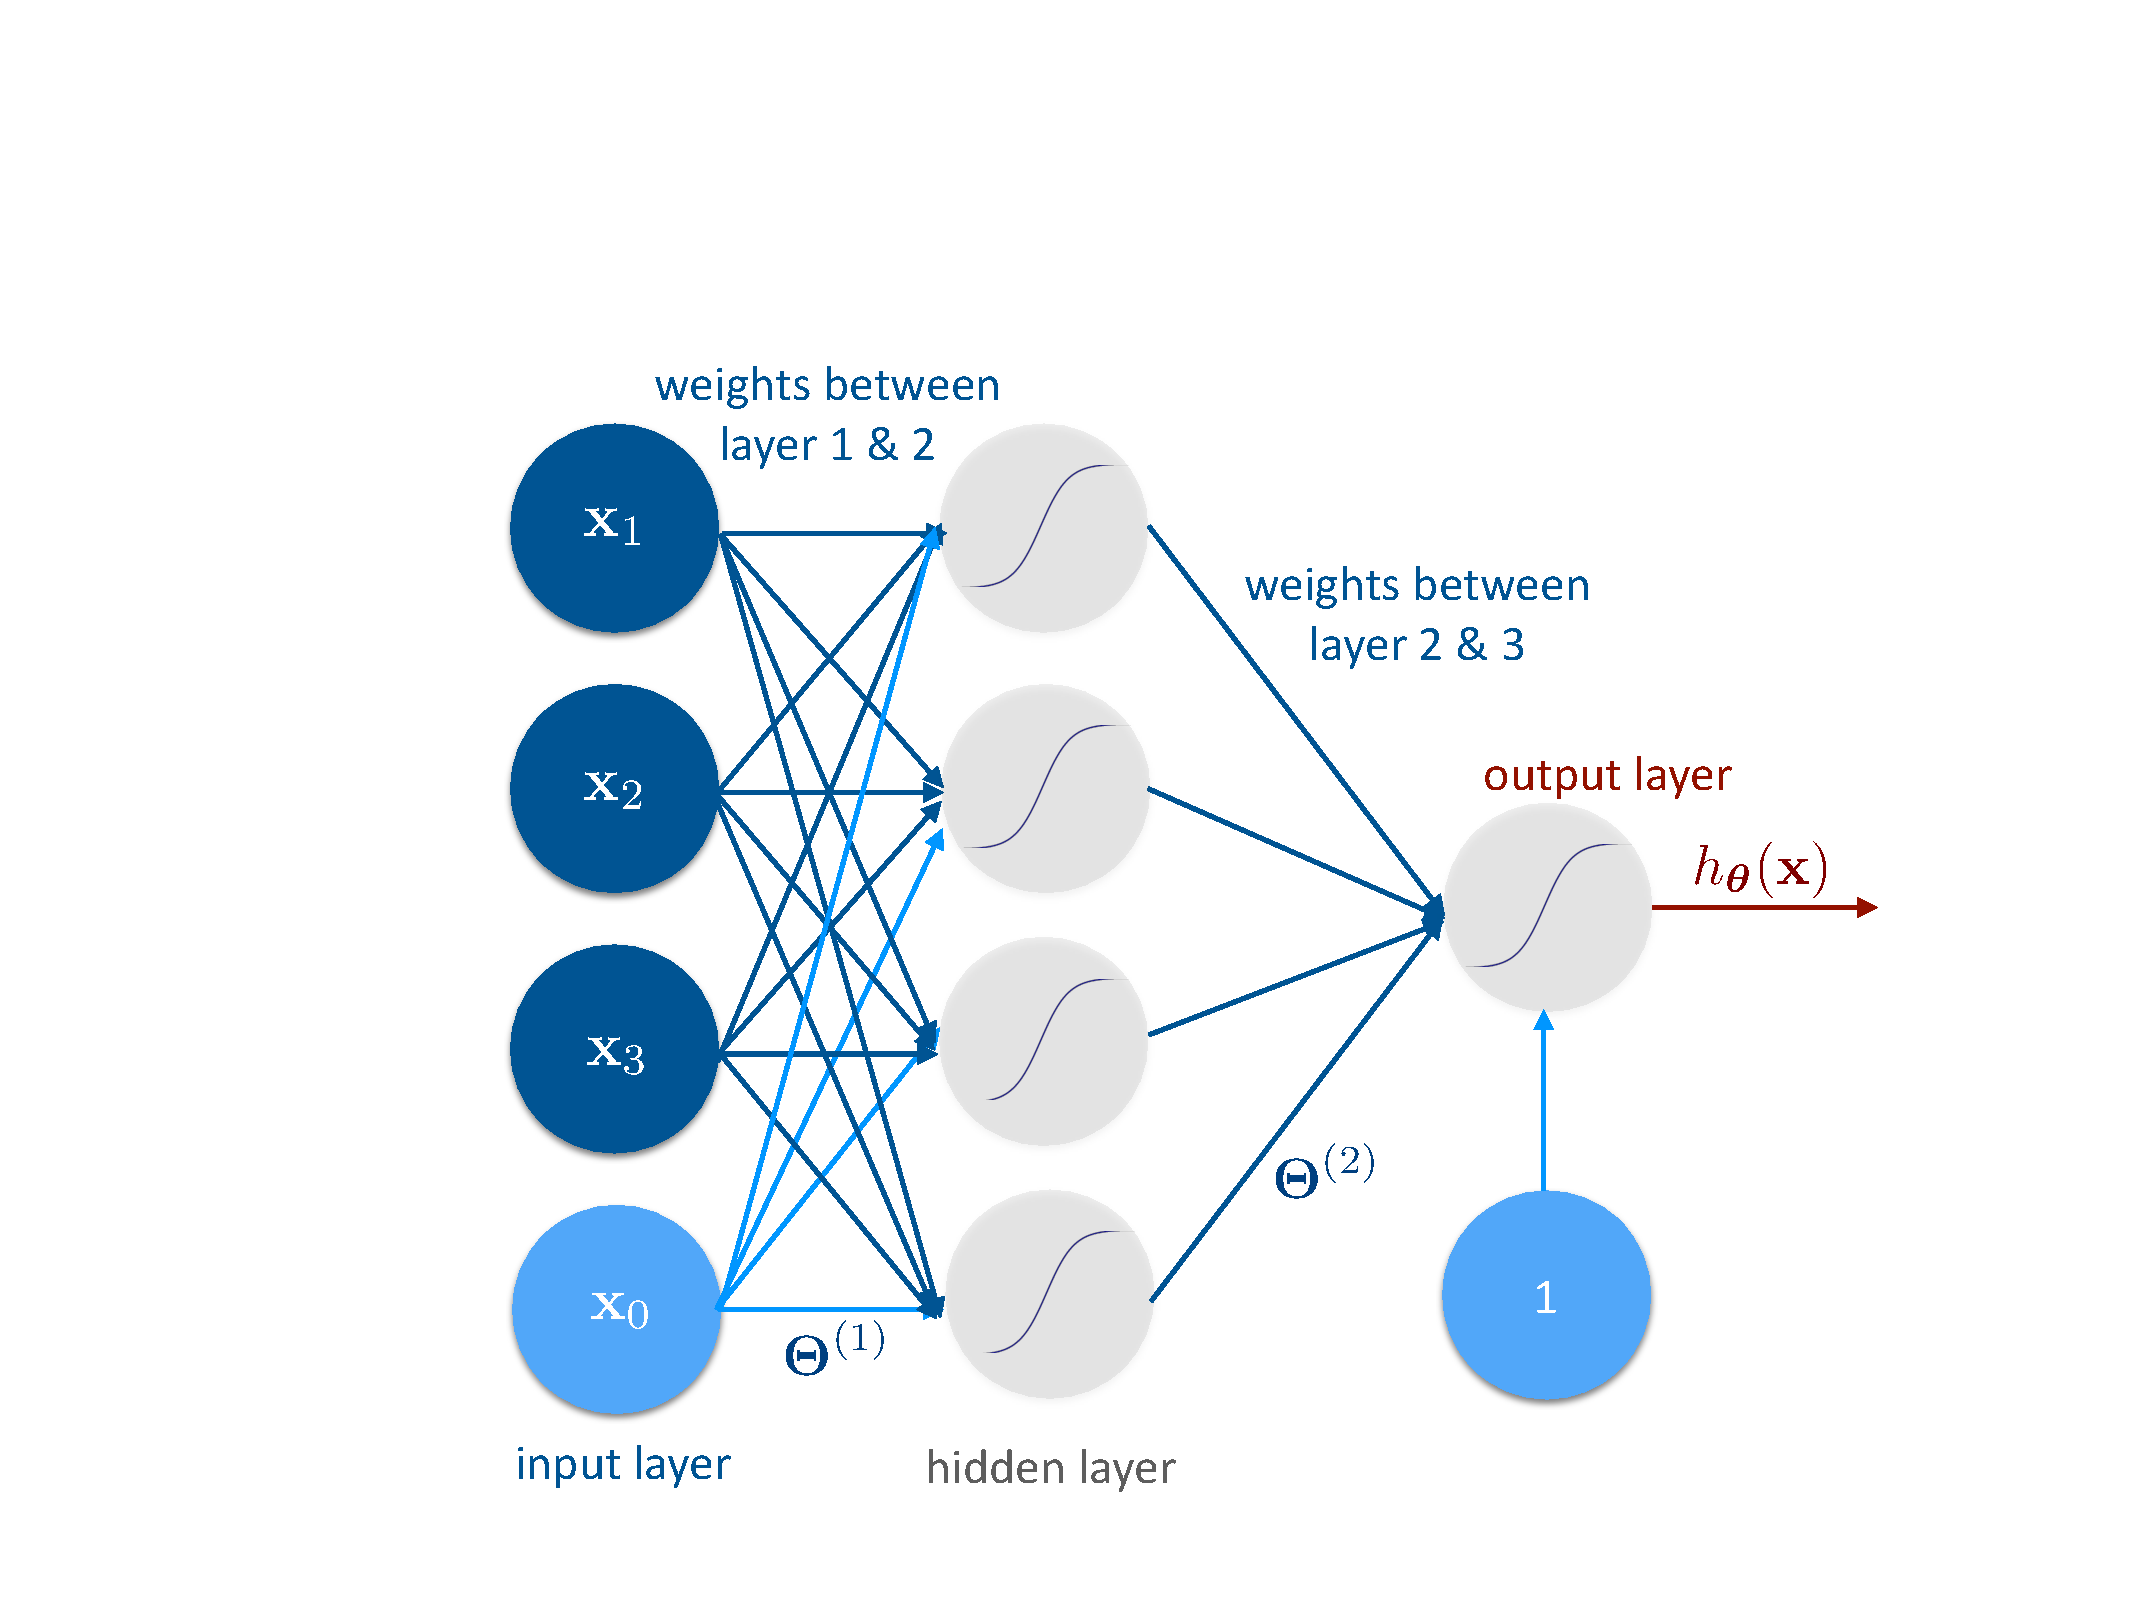
\includegraphics[trim = 10em 1em 10em 10em, clip, scale=.3]{NN}
\caption{A high-level depiction of an artificial neural network showing three layers as well as the weight connections between them.}
\end{figure}
To better understand the above notation, let us reconsider the example of Figure~\ref{Fig:FigTwo}. Specifically, let us illustrate the dimensionality and meaning of $\bm{\Theta}^{(1)}$, which connects layers one and two (i.e., input to hidden layer connections). It is easy to see that the input layer consists of three units and a bias, while the hidden layer of four sigmoidal units. Hence, the dimensionality of $\bm{\Theta}^{(1)}$ is given by $4 \times (3+1)$. In other words, the row-count of $\bm{\Theta}$ is given by the number of units in the successor layer (i.e., layer $l+1$), while the column-count by the number of units in the current layer (i.e., $l$) appended by an additional dimension for the bias term:
\begin{equation*}
\bm{\Theta}^{(1)} = \left[\begin{array}{cccc}
\bm{\Theta}^{(1)}_{10} & \bm{\Theta}^{(1)}_{11} & \bm{\Theta}^{(1)}_{12} & \bm{\Theta}^{(1)}_{13} \\
\bm{\Theta}^{(1)}_{20} & \bm{\Theta}^{(1)}_{21} & \bm{\Theta}^{(1)}_{22} & \bm{\Theta}^{(1)}_{23} \\
\bm{\Theta}^{(1)}_{30} & \bm{\Theta}^{(1)}_{31} & \bm{\Theta}^{(1)}_{32} & \bm{\Theta}^{(1)}_{33} \\
\bm{\Theta}^{(1)}_{40} & \bm{\Theta}^{(1)}_{41} & \bm{\Theta}^{(1)}_{42} & \bm{\Theta}^{(1)}_{43} \\
\end{array}
\right].
\end{equation*} 
If we consider row one in $\bm{\Theta}^{(1)}$, for example, we come to recognize that it corresponds to representing the connections between all the nodes from the input layer (i.e., $l=1$) to the \emph{first} node in the hidden (i.e., when $l=2$). Hence, $\bm{\Theta}^{(l)}_{ij}$ denotes the connecting weight initiating from node $j$ in layer $l$ to node $i$ in layer $l+1$, see Figure~\ref{Fig:FigThree} for a pictorial illustration. 

\begin{figure}[h!]
\label{Fig:FigThree}
\centering 
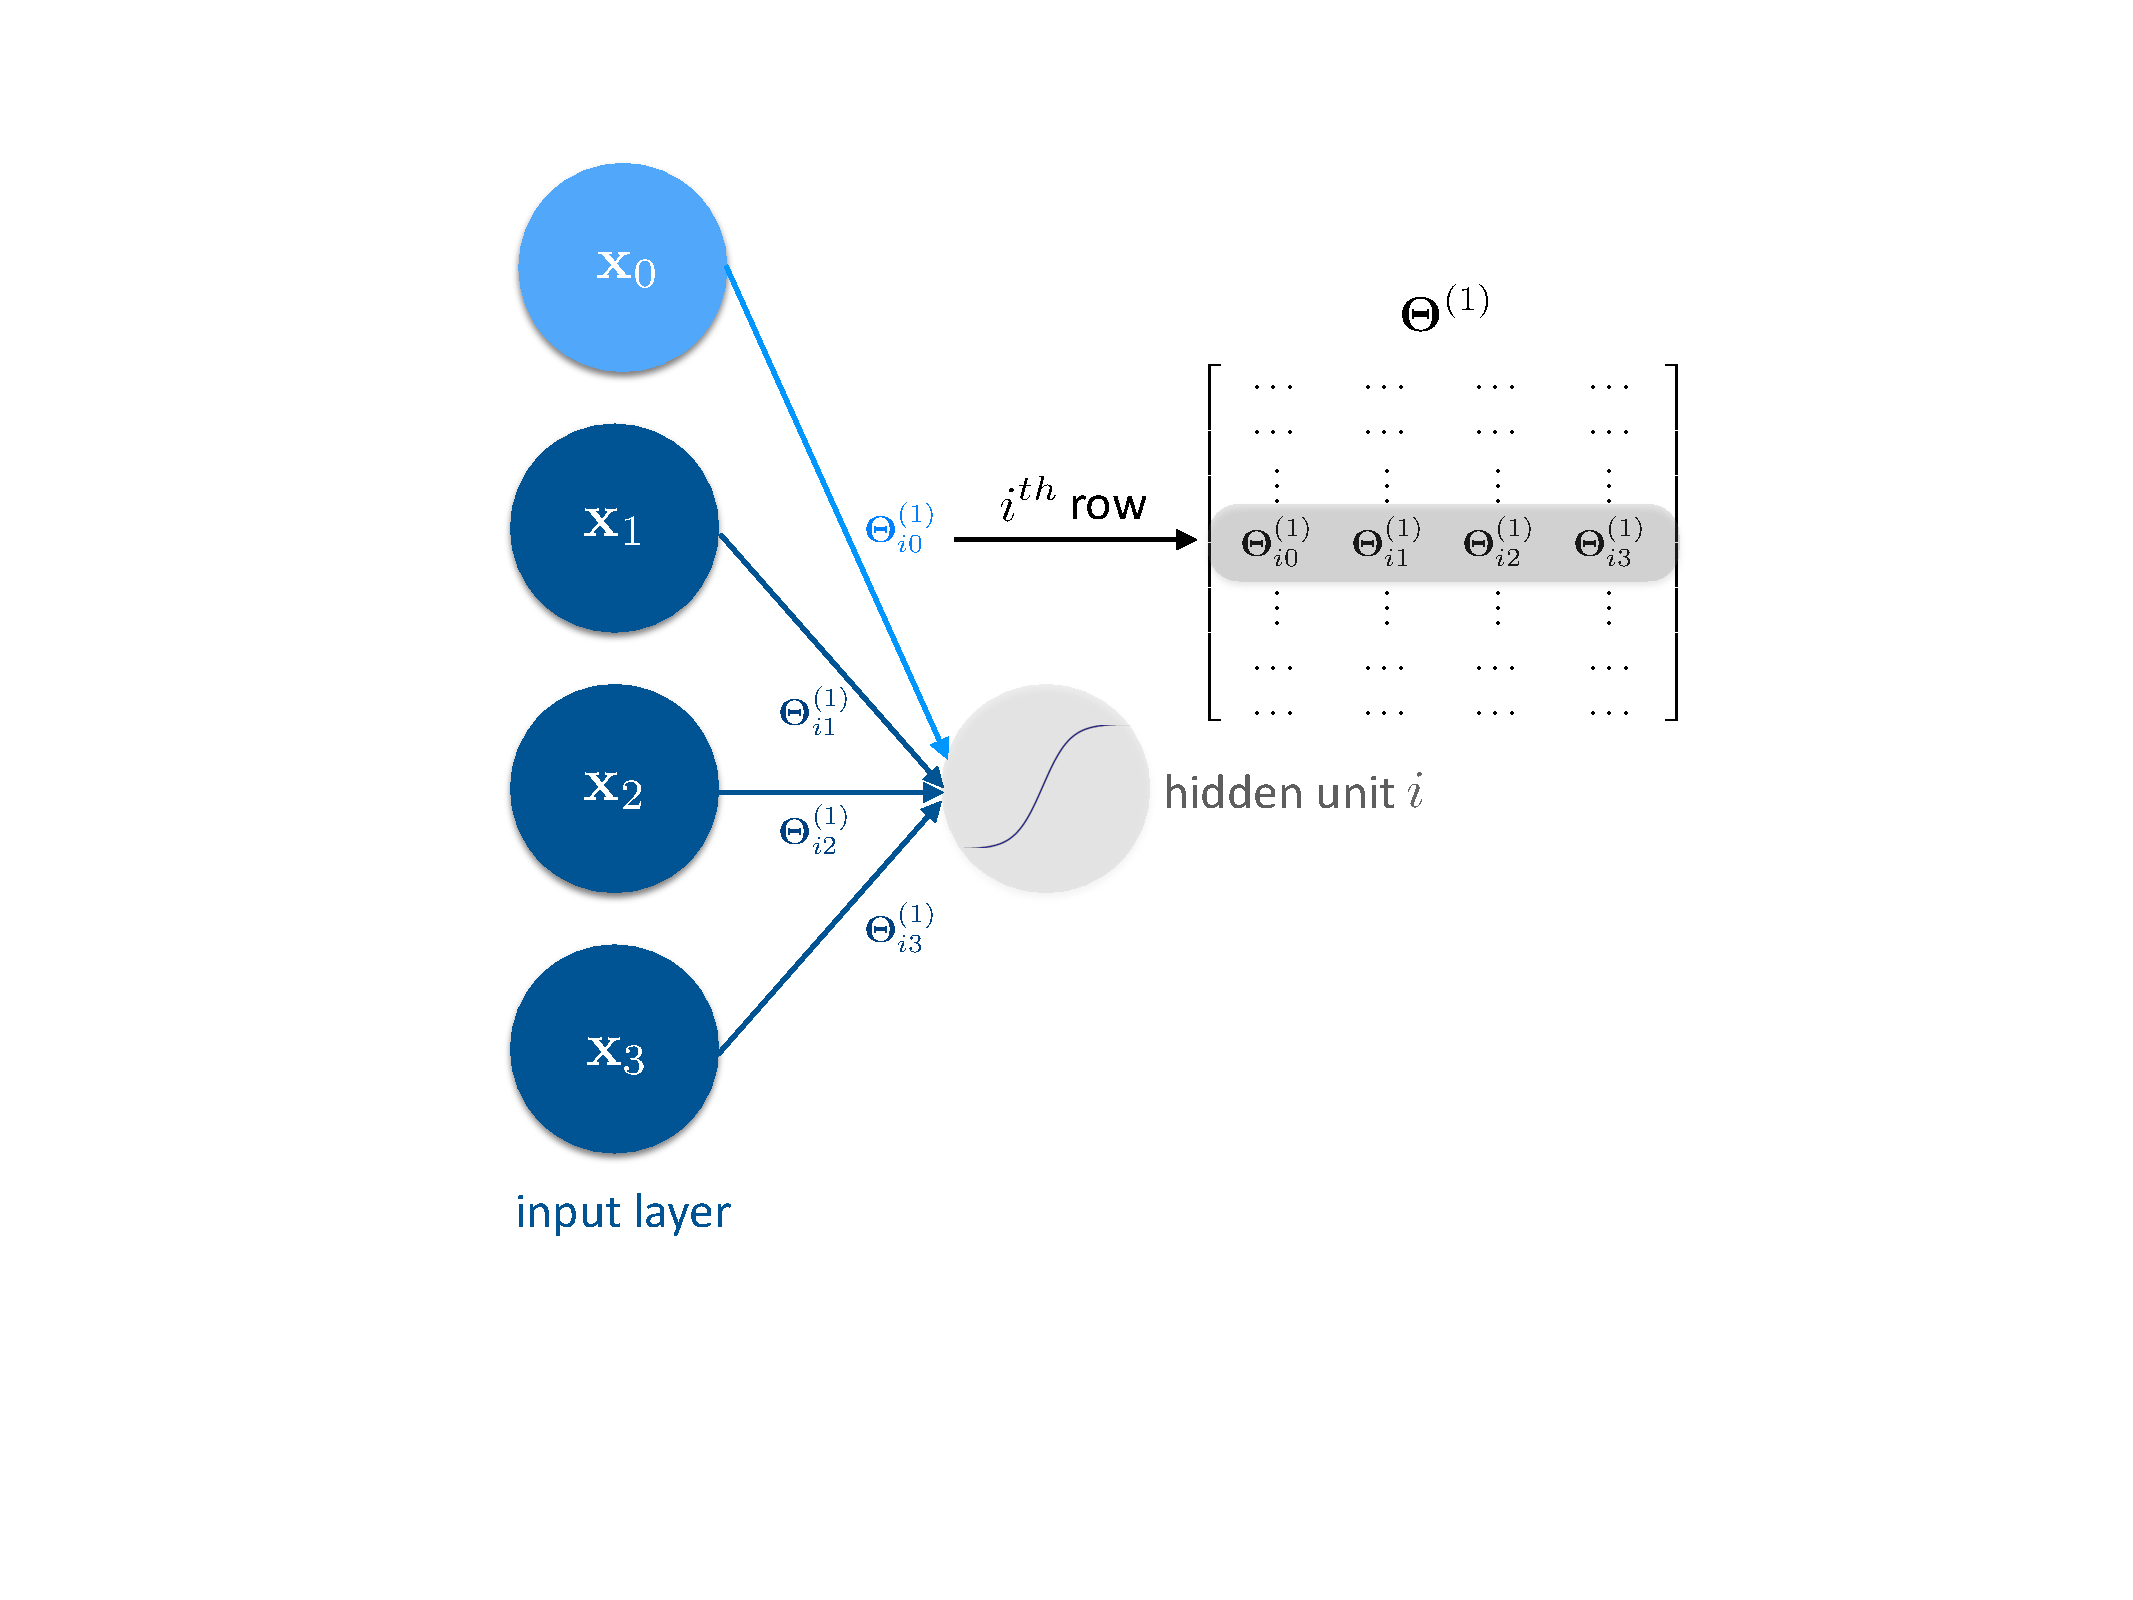
\includegraphics[trim = 10em 10em 10em 1em, clip, scale=.4]{OneUnitTheta}
\caption{An illustration of the weights connecting the units in the input layer to unit $i$ in the hidden layer.}
\end{figure}
\subsection{Feed Forward Propagation}\label{Sec:Notation}
Given the notation introduced above, we are now ready to discuss the computations that are performed by a neural network. Intuitively, between every two layers the inputs from the previous layer are, first, linearly (through the weight matrices) propagated forward and then nonlinearly transformed (through the sigmoids) to produce an output on the successor layer. Recursing this process, which we refer to as forward propagation, over the total layers of the network will produce an output on the final layer $L$. In what comes next, we will present an efficient vectorized implementation of forward propagation. 

We call the computation performed by node $i$ in layer $l$ an activation and denote it by $a_{i}^{(l)}= \text{sigmoid}\left(\sum_{j=0}^{s_{l-1}}\bm{\Theta}^{(l-1)}_{ij}a_{j}^{(l-1)}\right)$, with $a_{0}^{(l-1)} = 1$, and $a_{j}^{(l-1)}$ for $j \in \{1,\dots, s_{l-1}\}$ being the activations of the previous layer provided that the activations of the input (or first layer) are the data points themselves. Clearly, $a_{i}^{(l)}$ can be written in a matrix-vector product form with the help of $\bm{\Theta}^{(l-1)}$. Essentially, the input to the sigmoidal function is a linear combination between the $i^{th}$ row of the weight matrix and the activations on the previous layer: 
\begin{equation*}
a_{i}^{(l)} = \text{sigmoid}\left(\bm{\Theta}^{(l-1), \mathsf{T}}_{i,:} \bm{a}^{(l-1)}\right) = \frac{1}{1+ e^{-\bm{\Theta}^{(l-1), \mathsf{T}}_{i,:} \bm{a}^{(l-1)}}},
\end{equation*}
where $\bm{\Theta}^{(l-1), \mathsf{T}}_{i,:}$ denotes the $i^{th}$ row of $\bm{\Theta}^{(l-1)}$, and $\bm{a}^{(l-1)}$ is a vector collecting all activations (including that of the bias term) of layer $l-1$, i.e., $\bm{a}^{(l-1)} = \left[1, a_{1}^{(l-1)}, a_{2}^{(l-1)}, \dots, a_{s_{l-1}}^{(l-1)}\right]^{\mathsf{T}}$. Now, we can easily generalize the above notion to compute the activations in layer $l$  by considering the whole matrix $\bm{\Theta}^{(l-1)}$: 
\begin{align*}
\bm{a}^{(l)} & = \text{sigmoid} \left(\bm{\Theta}^{(l-1)}\bm{a}^{(l-1)}\right) \\
& = \text{sigmoid} \left[\left(\begin{array}{cccc}
\bm{\Theta}_{10}^{(l-1)} & \bm{\Theta}_{12}^{(l-1)} & \dots & \bm{\Theta}_{1s_{l-1}}^{(l-1)} \\
\bm{\Theta}_{20}^{(l-1)} & \bm{\Theta}_{21}^{(l-1)} & \dots & \bm{\Theta}_{2s_{l-1}}^{(l-1)} \\ 
\vdots & \vdots & \vdots & \vdots \\
\bm{\Theta}_{s_{l+1}0}^{(l-1)} & \bm{\Theta}_{s_{l+1}1}^{(l-1)} & \dots & \bm{\Theta}_{s_{l+1}s_{l-1}}^{(l-1)} \\ 
\end{array}
\right)\left[\begin{array}{c}
1 \\
a_{1}^{(l-1)} \\
\vdots \\
a_{s_{l-1}}^{(l-1)} \\
\end{array}
\right]\right] \\
& = \left[\begin{array}{c}
\text{sigmoid}\left(\bm{\Theta}^{(l-1), \mathsf{T}}_{1,:} \bm{a}^{(l-1)}\right)
 \\
 \text{sigmoid}\left(\bm{\Theta}^{(l-1), \mathsf{T}}_{2,:} \bm{a}^{(l-1)}\right) \\
 \vdots \\
 \text{sigmoid}\left(\bm{\Theta}^{(l-1), \mathsf{T}}_{s_{l+1},:} \bm{a}^{(l-1)}\right) 
\end{array} 
\right].
\end{align*}


To illustrate, consider the problem of performing classification that differentiates between four (or $K$) classes. To do so, we are going to change the architecture of the network to produce a four-dimensional output. This can be achieved by constructing a network with four output units as depicted in Figure~\ref{Fig:Network}. Here, we also chose to introduce an additional hidden layer hoping to learn more descriptive features. 


\begin{figure}[h!]
\centering 
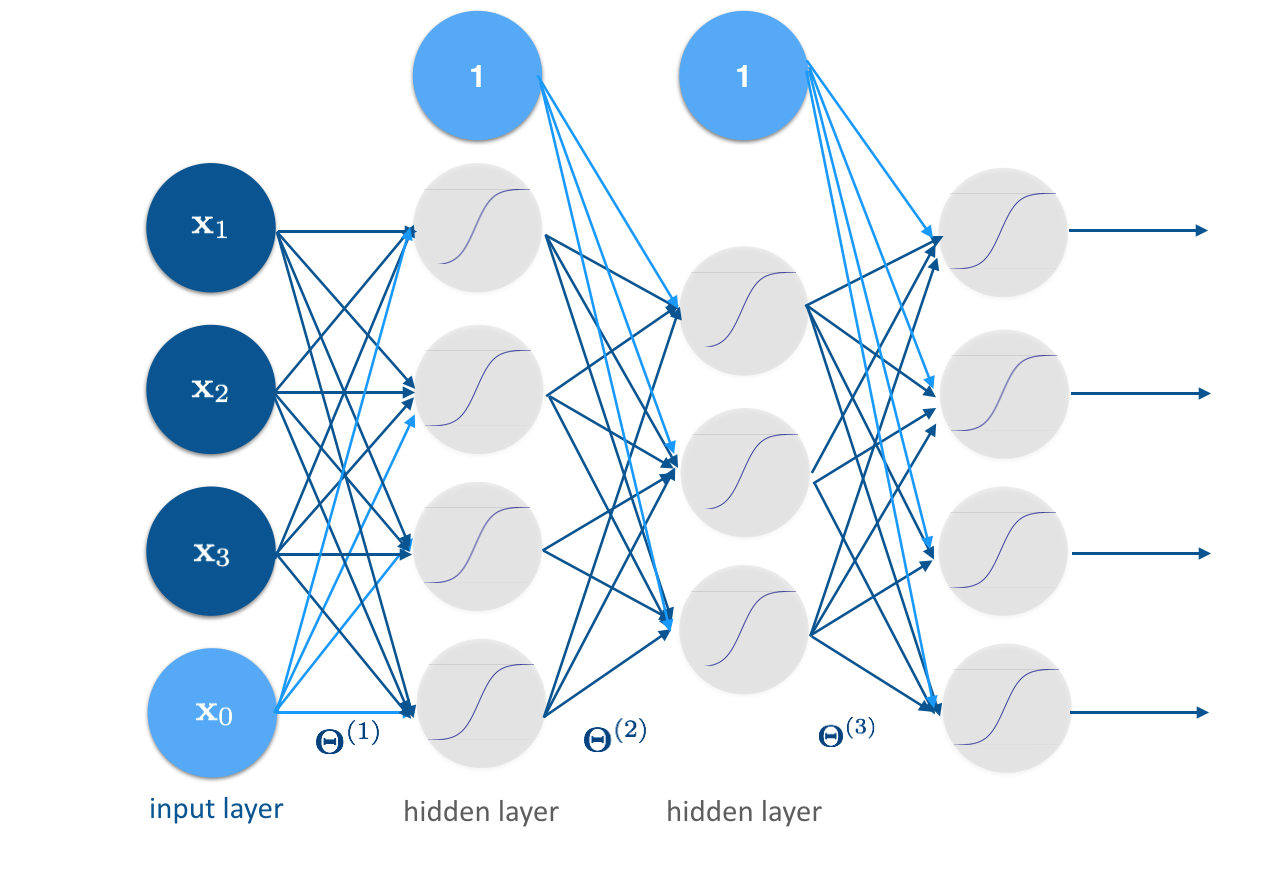
\includegraphics[scale=.5]{Network}
\caption{A high-level depiction of an artificial neural network showing four layers as well as the weight connections between them.}
\label{Fig:Network}
\end{figure}

This network has an input, 2 hidden, and an output layer. Given that we have 4 layers in total, we need three weight matrices (i.e., $\bm{\Theta}^{(1)}$, $\bm{\Theta}^{(2)}$, and $\bm{\Theta}^{(3)}$) to denote the connections among them. The dimensions of these weights can be determined as follows: 
\begin{equation*}
\bm{\Theta}^{(1)} \in \mathbb{R}^{4 \times 4}, \ \ \ \ \bm{\Theta}^{(2)} \in \mathbb{R}^{3 \times 5}, \ \ \ \ \  \bm{\Theta}^{(3)} \in \mathbb{R}^{4 \times 4}. 
\end{equation*}
As detailed previously, during feed-forward propagation, our goal is to determine the activations on each of the layers. The activations of the input layer are set to the input data themselves in addition to a bias term. That is: 
\begin{equation*}
\bm{a}^{(1)} = \left[\begin{array}{c}
1\\
\bm{x}_{1}\\
\bm{x}_{2}\\
\bm{x}_{3}
\end{array}
\right].
\end{equation*}
Given, $\bm{\Theta}^{(1)}$, we can now compute an intermediate vector $\bm{z}^{(2)}$, which will be used to determine the activations on the second layer (i.e., first hidden layer) that are denoted by $\bm{a}^{(2)}$:

\begin{equation*}
\bm{z}^{(2)} = \underbrace{\bm{\Theta}^{(1)}}_{\in \mathbb{R}^{4 \times 4}}\overbrace{\bm{a}^{(1)}}^{\in \mathbb{R}^{4 \times 1}} \ \ \ \ \implies \bm{a}^{(2)} =\text{sigmoid}(\bm{z}^{(2)}) = \text{sigmoid}\left(\bm{\Theta}^{(1)}\bm{a}^{(1)}\right). 
\end{equation*}
Given, $\bm{a}^{(2)}$, we can continue our recursion to determine the activations on each of the successor layers. Note, however, that at each layer we need to append an additional dimension for the bias term. In other words, create $\bm{a}^{(2)} = [1, a^{(2)}_{1}, a^{(2)}_{2}, a^{(2)}_{3}, a^{(2)}_{4}]^{\mathsf{T}}$, and the perform: 
\begin{align*}
\bm{z}^{(3)} &= \underbrace{\bm{\Theta}^{(2)}}_{\in \mathbb{R}^{3 \times 5}}\overbrace{\bm{a}^{(2)}}^{\in \mathbb{R}^{5 \times 1}} \ \ \ \ \implies \bm{a}^{(3)} = \text{sigmoid}(\bm{z}^{(3)}) \\
\bm{z}^{(4)} &= \underbrace{\bm{\Theta}^{(3)}}_{\in \mathbb{R}^{4 \times 4}}\overbrace{\bm{a}^{(3)}}^{\in \mathbb{R}^{4 \times 1}} \ \ \ \ \implies \bm{a}^{(3)} = \text{sigmoid}(\bm{z}^{(3)}) \ \ \ \text{(we already appended 1 to $\bm{a}^{(3)}$)}.
\end{align*}



Having described feed forward propagation, the next step is to detail the strategy by which neural networks determine the model parameters (i.e., the $\bm{\Theta}^{(l)}$ matrices). In standard regression or classification problems, back-propagation is the algorithm adopted. Given an input data point, back-propagation commences as follows. First, forward propagation is executed and the network is made to output a value. This value is then compared to the real output from the data set producing an error. This error is then propagated backwards to every other layer and used to update connecting weights. Such updates typically involve gradient-based methods (e.g., stochastic gradients). 

The process detailed so-far operates successfully for relatively ``shallow'' networks, i.e., networks with low number of hidden layers. As the number of these layers increases (i.e., deep neural network), propagating gradients backward becomes increasingly challenging leading to convergence to local minima. To circumvent the above problems, we adapt a solution by which gradient updates are not performed at each iteration of the training algorithm. In particular, we assume additional knowledge modelled via an alternative NN that encodes previously experienced traces. This NN is used as a reference that we update after a preset number of iterations. As such, old knowledge encountered by the agent is not hindered by novel observations. 
